%
%Не забыть:
%--------------------------------------
%Вставить колонтитулы, поменять название на титульнике



%--------------------------------------

\documentclass[a4paper, 12pt]{article} 

%--------------------------------------
%Russian-specific packages
%--------------------------------------
%\usepackage[warn]{mathtext}
\usepackage[T2A]{fontenc}
\usepackage[utf8]{inputenc}
\usepackage[english,russian]{babel}
\usepackage[intlimits]{amsmath}
\usepackage{esint}
%--------------------------------------
%Hyphenation rules
%--------------------------------------
\usepackage{hyphenat}
\hyphenation{ма-те-ма-ти-ка вос-ста-нав-ли-вать}
%--------------------------------------
%Packages
%--------------------------------------
\usepackage{amsmath}
\usepackage{amssymb}
\usepackage{amsfonts}
\usepackage{amsthm}
\usepackage{latexsym}
\usepackage{mathtools}
\usepackage{etoolbox}%Булевые операторы
\usepackage{extsizes}%Выставление произвольного шрифта в \documentclass
\usepackage{geometry}%Разметка листа
\usepackage{indentfirst}
\usepackage{wrapfig}%Создание обтекаемых текстом объектов
\usepackage{fancyhdr}%Создание колонтитулов
\usepackage{setspace}%Настройка интерлиньяжа
\usepackage{lastpage}%Вывод номера последней страницы в документе, \lastpage
\usepackage{soul}%Изменение параметров начертания
\usepackage{hyperref}%Две строчки с настройкой гиперссылок внутри получаеммого
\usepackage[usenames,dvipsnames,svgnames,table,rgb]{xcolor}% pdf-документа
\usepackage{multicol}%Позволяет писать текст в несколько колонок
\usepackage{cite}%Работа с библиографией
\usepackage{subfigure}% Человеческая вставка нескольких картинок
\usepackage{tikz}%Рисование рисунков
\usepackage{float}% Возможность ставить H в положениях картинки
% Для картинок Моти
\usepackage{misccorr}
\usepackage{lscape}
\usepackage{cmap}

\usepackage{mhchem}



\usepackage{graphicx,xcolor}
\graphicspath{{Pictures/}}
\DeclareGraphicsExtensions{.pdf,.png,.jpg}

%----------------------------------------
%Список окружений
%----------------------------------------
\newenvironment {theor}[2]
{\smallskip \par \textbf{#1.} \textit{#2}  \par $\blacktriangleleft$}
{\flushright{$\blacktriangleright$} \medskip \par} %лемма/теорема с доказательством
\newenvironment {proofn}
{\par $\blacktriangleleft$}
{$\blacktriangleright$ \par} %доказательство
%----------------------------------------
%Список команд
%----------------------------------------
\newcommand{\grad}
{\mathop{\mathrm{grad}}\nolimits\,} %градиент

\newcommand{\diver}
{\mathop{\mathrm{div}}\nolimits\,} %дивергенция

\newcommand{\rot}
{\ensuremath{\mathrm{rot}}\,}

\newcommand{\Def}[1]
{\underline{\textbf{#1}}} %определение

\newcommand{\RN}[1]
{\MakeUppercase{\romannumeral #1}} %римские цифры

\newcommand {\theornp}[2]
{\textbf{#1.} \textit{ #2} \par} %Написание леммы/теоремы без доказательства

\newcommand{\qrq}
{\ensuremath{\quad \Rightarrow \quad}} %Человеческий знак следствия

\newcommand{\qlrq}
{\ensuremath{\quad \Leftrightarrow \quad}} %Человеческий знак равносильности

\renewcommand{\phi}{\varphi} %Нормальный знак фи

\newcommand{\me}
{\ensuremath{\mathbb{E}}}

\newcommand{\md}
{\ensuremath{\mathbb{D}}}



%\renewcommand{\vec}{\overline}




%----------------------------------------
%Разметка листа
%----------------------------------------
\geometry{top = 3cm}
\geometry{bottom = 2cm}
\geometry{left = 1.5cm}
\geometry{right = 1.5cm}
%----------------------------------------
%Колонтитулы
%----------------------------------------
\pagestyle{fancy}%Создание колонтитулов
\fancyhead{}
%\fancyfoot{}
\fancyhead[R]{\textsc{Спектрометрия}}%Вставить колонтитул сюда
%----------------------------------------
%Интерлиньяж (расстояния между строчками)
%----------------------------------------
%\onehalfspacing -- интерлиньяж 1.5
%\doublespacing -- интерлиньяж 2
%----------------------------------------
%Настройка гиперссылок
%----------------------------------------
\hypersetup{				% Гиперссылки
	unicode=true,           % русские буквы в раздела PDF
	pdftitle={Заголовок},   % Заголовок
	pdfauthor={Автор},      % Автор
	pdfsubject={Тема},      % Тема
	pdfcreator={Создатель}, % Создатель
	pdfproducer={Производитель}, % Производитель
	pdfkeywords={keyword1} {key2} {key3}, % Ключевые слова
	colorlinks=true,       	% false: ссылки в рамках; true: цветные ссылки
	linkcolor=blue,          % внутренние ссылки
	citecolor=blue,        % на библиографию
	filecolor=magenta,      % на файлы
	urlcolor=blue           % на URL
}
%----------------------------------------
%Работа с библиографией (как бич)
%----------------------------------------
\renewcommand{\refname}{Список литературы}%Изменение названия списка литературы для article
%\renewcommand{\bibname}{Список литературы}%Изменение названия списка литературы для book и report
%----------------------------------------
\begin{document}
	\begin{titlepage}
		\begin{center}
			$$$$
			$$$$
			$$$$
			$$$$
			{\Large{НАЦИОНАЛЬНЫЙ ИССЛЕДОВАТЕЛЬСКИЙ УНИВЕРСИТЕТ}}\\
			\vspace{0.1cm}
			{\Large{ВЫСШАЯ ШКОЛА ЭКОНОМИКИ}}\\
			\vspace{0.25cm}
			{\large{Факультет физики}}\\
			\vspace{5.5cm}
			{\Huge\textbf{{Лабораторная работа}}}\\%Общее название
			\vspace{1cm}
			{\LARGE{<<Спектрометрия>>}}\\%Точное название
			\vspace{2cm}
			{Работу выполнил студент 3 курса}\\
			{Захаров Сергей Дмитриевич}
			\vfill
			
\includegraphics[width = 0.2\textwidth]{HSElogo}\\
			\vfill
			Москва\\
			2020
		\end{center}
	\end{titlepage}
	
\tableofcontents

\newpage

\section{Цели работы}

Перед началом выполнения работы нами были поставлены следующие цели:

\begin{itemize}
	\item Ознакомиться с принципом работы с представленным спектрометром.
	
	\item Получить с его помощью спектры излучения различных ламп (\ce{H2}, \ce{He}, \ce{Ar}, \ce{Hg}, \ce{Kr}, \ce{Ne}, \ce{Na})
	
	\item Изучить Рамановские спектры некоторых подручных веществ.
	
	\item Провести измерение спектра Солнца (или неба) напрямую и через стекло. Получить на основании этих данных функцию пропускания стекла.
\end{itemize}

\section{Спектры излучения ламп}

Схема установки приведена на рисунке \ref{fig:spectrometer}. Заявленная погрешность спектрометра составляет 0.7~nм.


\begin{figure}[H]
	\centering
	\includegraphics[width=0.7\linewidth]{spectrometer.png}
	\caption{Установка состоит из источника питания (1), на корпусе которого находится держатель газоразрядной трубки (2), и спектрометра (3) с оптоволоконным кабелем, подводящим излучение к спектральному прибору.}
	\label{fig:spectrometer}
\end{figure}

\subsection{Спектр \ce{Ar}}

Полученный спектр приведен на рисунке \ref{fig:ar}. В ходе измерения были установлены заметные пики, представленные в таблице ниже:

\begin{center}
	\begin{tabular}{|c|c|c|c|c|}
		\hline
		Длина волны, nm & 416.0 & 420.1 & 696.8 & 707.0 \\
		\hline
		Табличная длина волны, nm & 415.9 & 420.0 & 696.5 & 706.9 \\
		\hline
	\end{tabular}
\end{center}






\subsection{Спектр \ce{He}}

Полученный спектр приведен на рисунке \ref{fig:he}. В ходе измерения были установлены заметные пики, представленные в таблице ниже:

\begin{center}
	\begin{tabular}{|c|c|c|c|c|c|}
		\hline
		Длина волны, nm & 447.3 & 501.8 & 589.9 & 668.2 & 706.9 \\
		\hline
		Табличная длина волны, nm & 447.2 & 501.6 & 587.6 & 668.0 & 706.6 \\
		\hline
	\end{tabular}
\end{center}






\subsection{Спектр \ce{Hg}}

Полученный спектр приведен на рисунке \ref{fig:hg}. В ходе измерения были установлены заметные пики, представленные в таблице ниже:

\begin{center}
	\begin{tabular}{|c|c|c|c|c|c|c|}
		\hline
		Длина волны, nm & 404.8 & 407.9 & 436.7 & 546.7 & 577.2 & 579.4 \\
		\hline
		Табличная длина волны, nm & 404.7 & 407.8 & 435.8 & 546.0 & 577.0 & 579.1 \\
		\hline
	\end{tabular}
\end{center}






\subsection{Спектр \ce{Kr}}

Полученный спектр приведен на рисунке \ref{fig:kr}. В ходе измерения были установлены заметные пики, представленные в таблице ниже:

\begin{center}
	\begin{tabular}{|c|c|c|c|c|}
		\hline
		Длина волны, nm & 427.6 & 432.2 & 557.4 & 587.3 \\
		\hline
		Табличная длина волны, nm & 427.4 & 432.3 & 557.3 & 587.4 \\
		\hline
	\end{tabular}
\end{center}






\subsection{Спектр \ce{Ne}}

Полученный спектр приведен на рисунке \ref{fig:ne}. В ходе эксперимента были получены сильно зашумленные данные, которые потребовали ручной обработки. После нее были получены следующие данные о пиках, представленные в таблице ниже:

\begin{center}
	\begin{tabular}{|c|c|c|c|}
		\hline
		Длина волны, nm & 585.5 & 614.5 & 650.9 \\
		\hline
		Табличная длина волны, nm & 585.2 & 614.3 & 650.7 \\
		\hline
	\end{tabular}
\end{center}





\subsection{Спектр \ce{H2}}

Полученный спектр приведен на рисунке \ref{fig:h2}. Данные имеют невероятно низкое качество и сильно зашумлены, что делает их очень слабо пригодными для обработки, однако наличие явного яркого пика на длине волны порядка 650~nм позволяет спорно, но все же утверждать, что перед нами действительно спектр водорода.




\subsection{Спектр \ce{Na}}

Полученный спектр приведен на рисунке \ref{fig:na}. В ходе измерения были установлены заметные пики (для места где должен быть дублет было взято среднее значение), представленные в таблице ниже:

\begin{center}
	\begin{tabular}{|c|c|c|c|c|}
		\hline
		Длина волны, nm & 568.6 & 569.2 & 589.27 & 616.3 \\
		\hline
		Табличная длина волны, nm & 568.3 & 568.8 & 588.995/589.592 & 615.4 \\
		\hline
	\end{tabular}
\end{center}

Отметим сразу, что расстояние между табличными линиями в дублете оказывается меньше, чем заявленная погрешность прибора, поэтому утверждать наверняка о наличии дублета в этом месте невозможно на чисто аппаратном уровне.




\section{Спектр Солнца (серого неба) и коэффициент пропускания оконного стекла}

В ходе экспериментов были получены спектры серого неба (спектр Солнца получить возможным не представлялось в силу погодных условий) напрямую и через оконное стекло. Имея оба спектра, при делении одного на другой получается интересующий нас график зависимости коэффициента пропускания оконного стекла от длины волны (по определению). Полученные данные представлены на графиках \ref{fig:sky} (спектр серого неба) и \ref{fig:glass_perm} (коэффициент пропускания). В целом последний график совпадает с тем, что мы предполагали получить: известно, что стекло не пропускает ультрафиолет и, разумеется, пропускает видимый свет, что и отражено на полученном нами графике. Видны также отличия спектра серого неба от ожидаемого нами спектра абсолютно черного тела, которым мы приближаем Солнце. Объясняется это в первую очередь рассеянием в атмосфере (в том числе и на облаках, важно понимать, что измерения проводились в пасмурную погоду), а также поглощения атмосферой излучения ряда длин волн (например, в ультрафиолетовой зоне).


\section{Рамановские спектры веществ}

В силу отсутствия у нас какого-либо каталога рамановских спектров, который бы включал в себя вещества, найденные нами на месте (а это были зеленка, вода, мел, кофеин в таблетках и валидол), сравнить полученные нами спектры с теми, которые можно было бы с достаточной уверенностью назвать табличными, не удалось, однако же с найденными нами фотографиями спектров (тех, которые мы найти смогли), они в целом совпадали. Полученные в ходе экспериментов данные представлены в виде графиках на рисунках \ref{fig:br_gr} (зеленка), \ref{fig:water} (вода), \ref{fig:chalk} (мел), \ref{fig:coffee} (кофеин в таблетках), \ref{fig:validol} (валидол).

\section{Выводы}

\begin{itemize}
	\item Было проведено ознакомление с представленными нам для работы спектрометрами.
	
	\item Были получены спектры представленных ламп, а также зарегистрированы длины волн, на которых достигается максимальная интенсивность их излучения. Полученные данные в целом совпали с табличными.
	
	\item Был получены спектры серого неба без стекла и с, на основании чего был получен график зависимости коэффициента пропускания оконного стекла в лаборатории от длины волны.
	
	\item Были получены рамановские спектры некоторых подручных веществ (зеленки, воды, мела, таблетки кофеина и валидола).
\end{itemize}

Данные по табличным длинам волн для различных материалов в 1 эксперименте были взяты здесь:  \href{https://www.physics.nist.gov/PhysRefData/ASD/lines_form.html}{https://www.physics.nist.gov/PhysRefData/ASD/lines\_form.html}.

% 1

\begin{figure}[H]
	\centering
	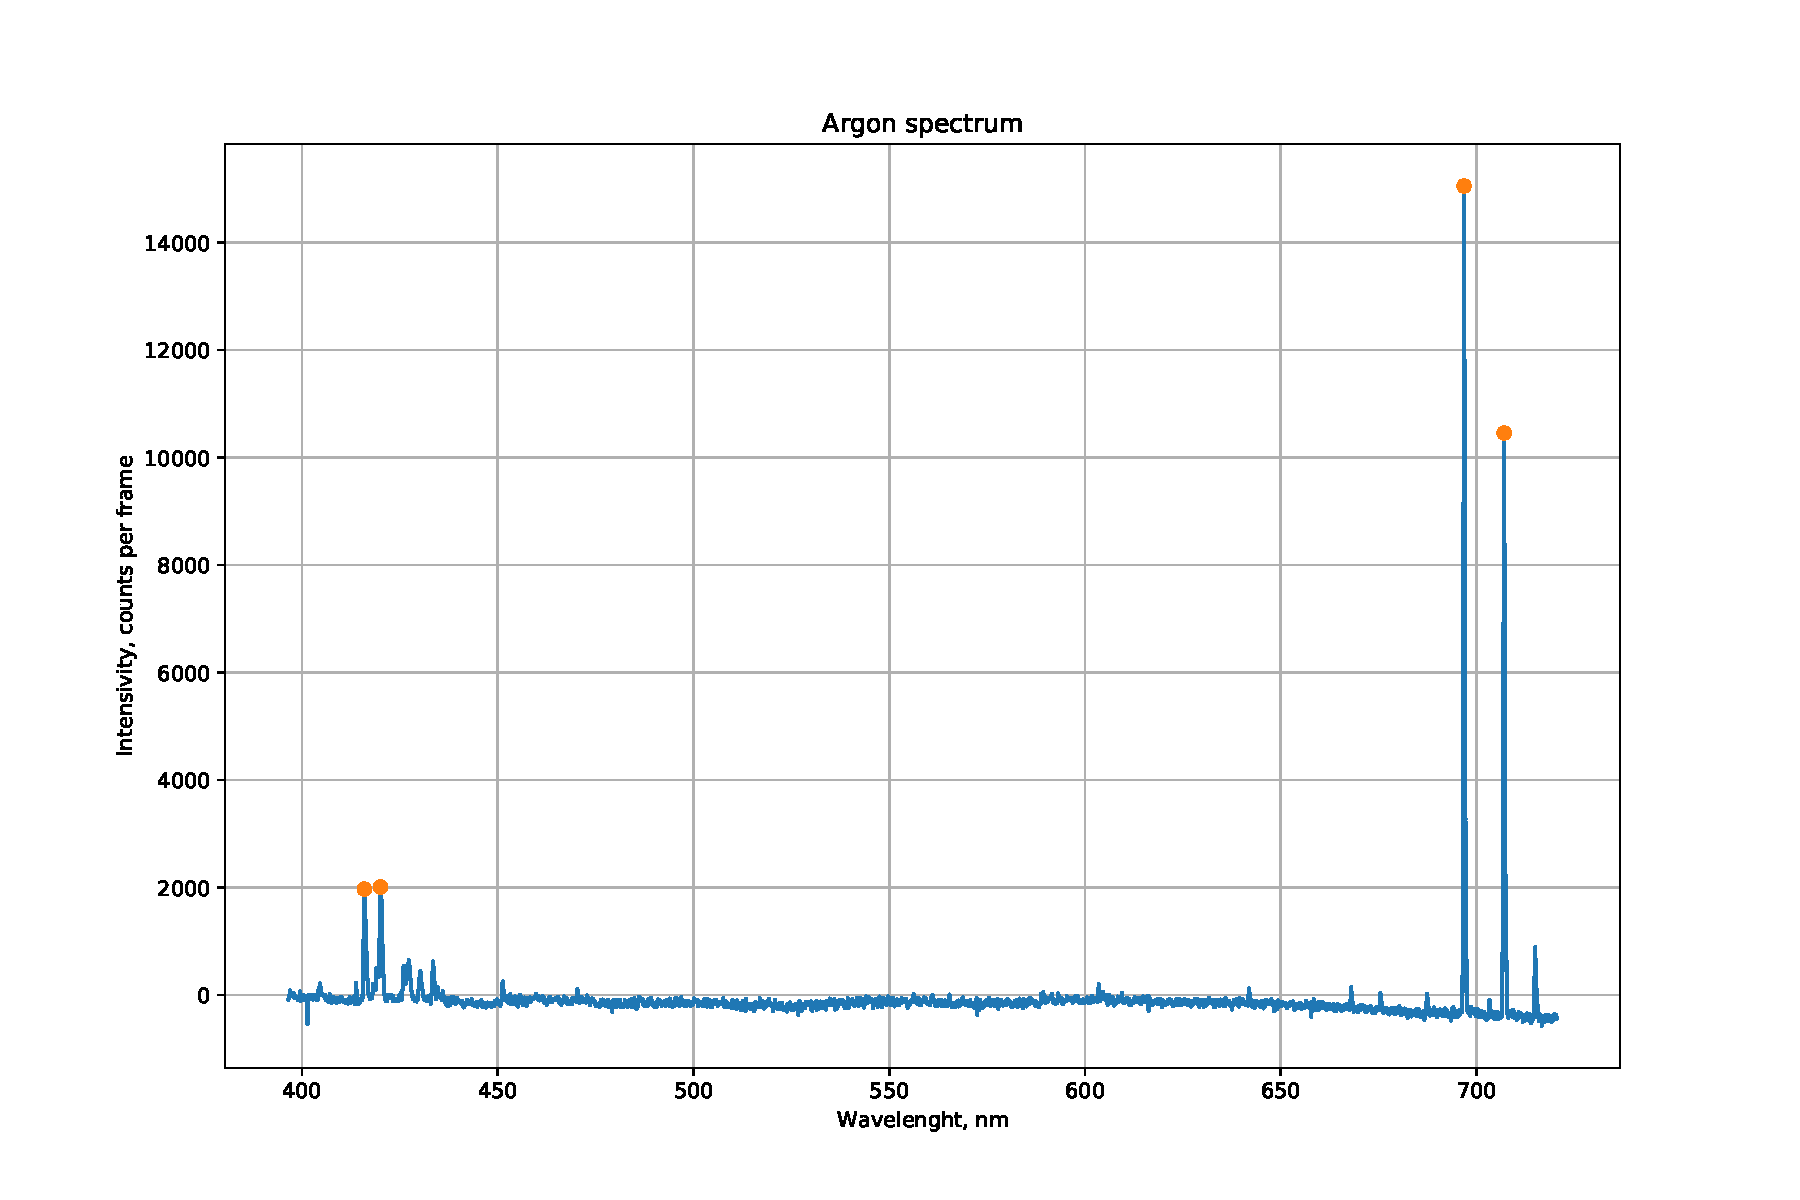
\includegraphics[width=0.9\linewidth]{argon}
	\caption{Спектр аргона}
	\label{fig:ar}
\end{figure}

\begin{figure}[H]
	\centering
	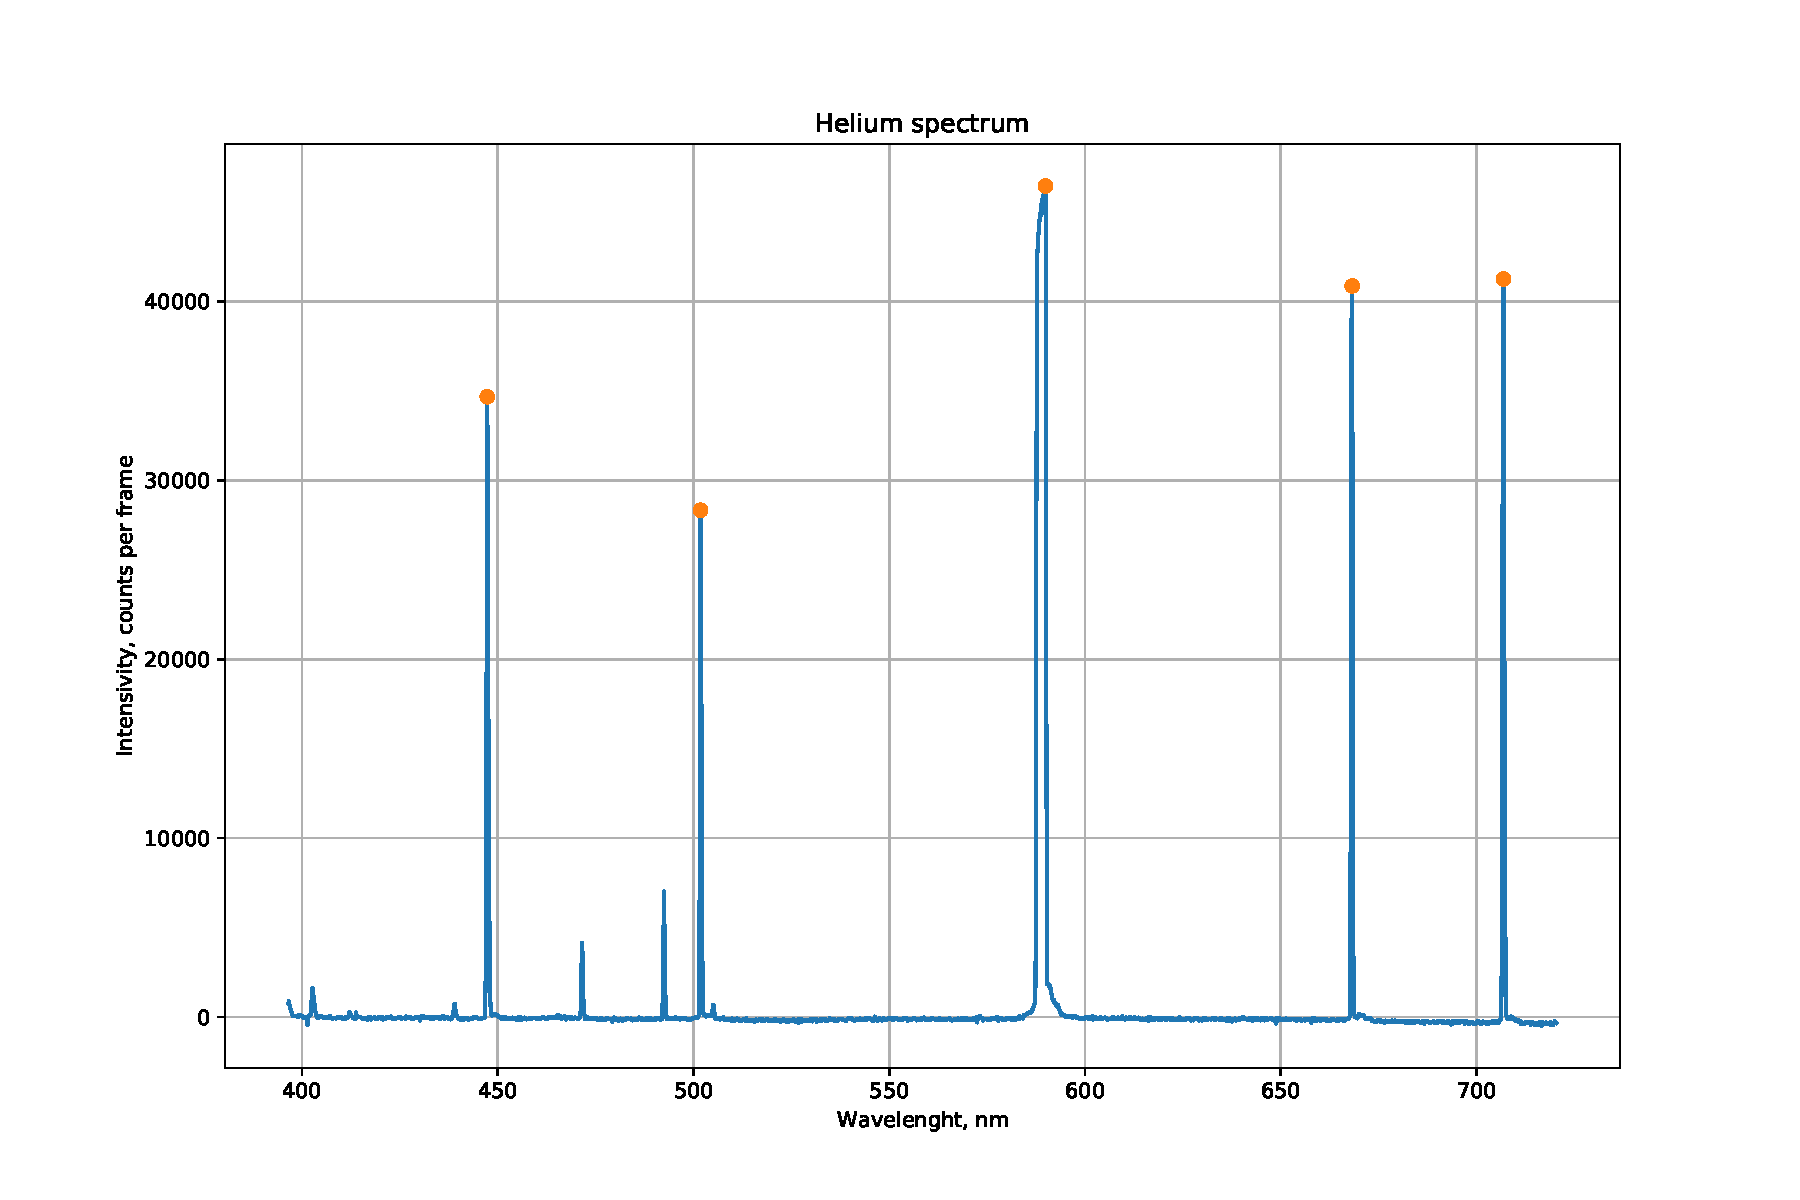
\includegraphics[width=0.9\linewidth]{helium}
	\caption{Спектр гелия}
	\label{fig:he}
\end{figure}

\begin{figure}[H]
	\centering
	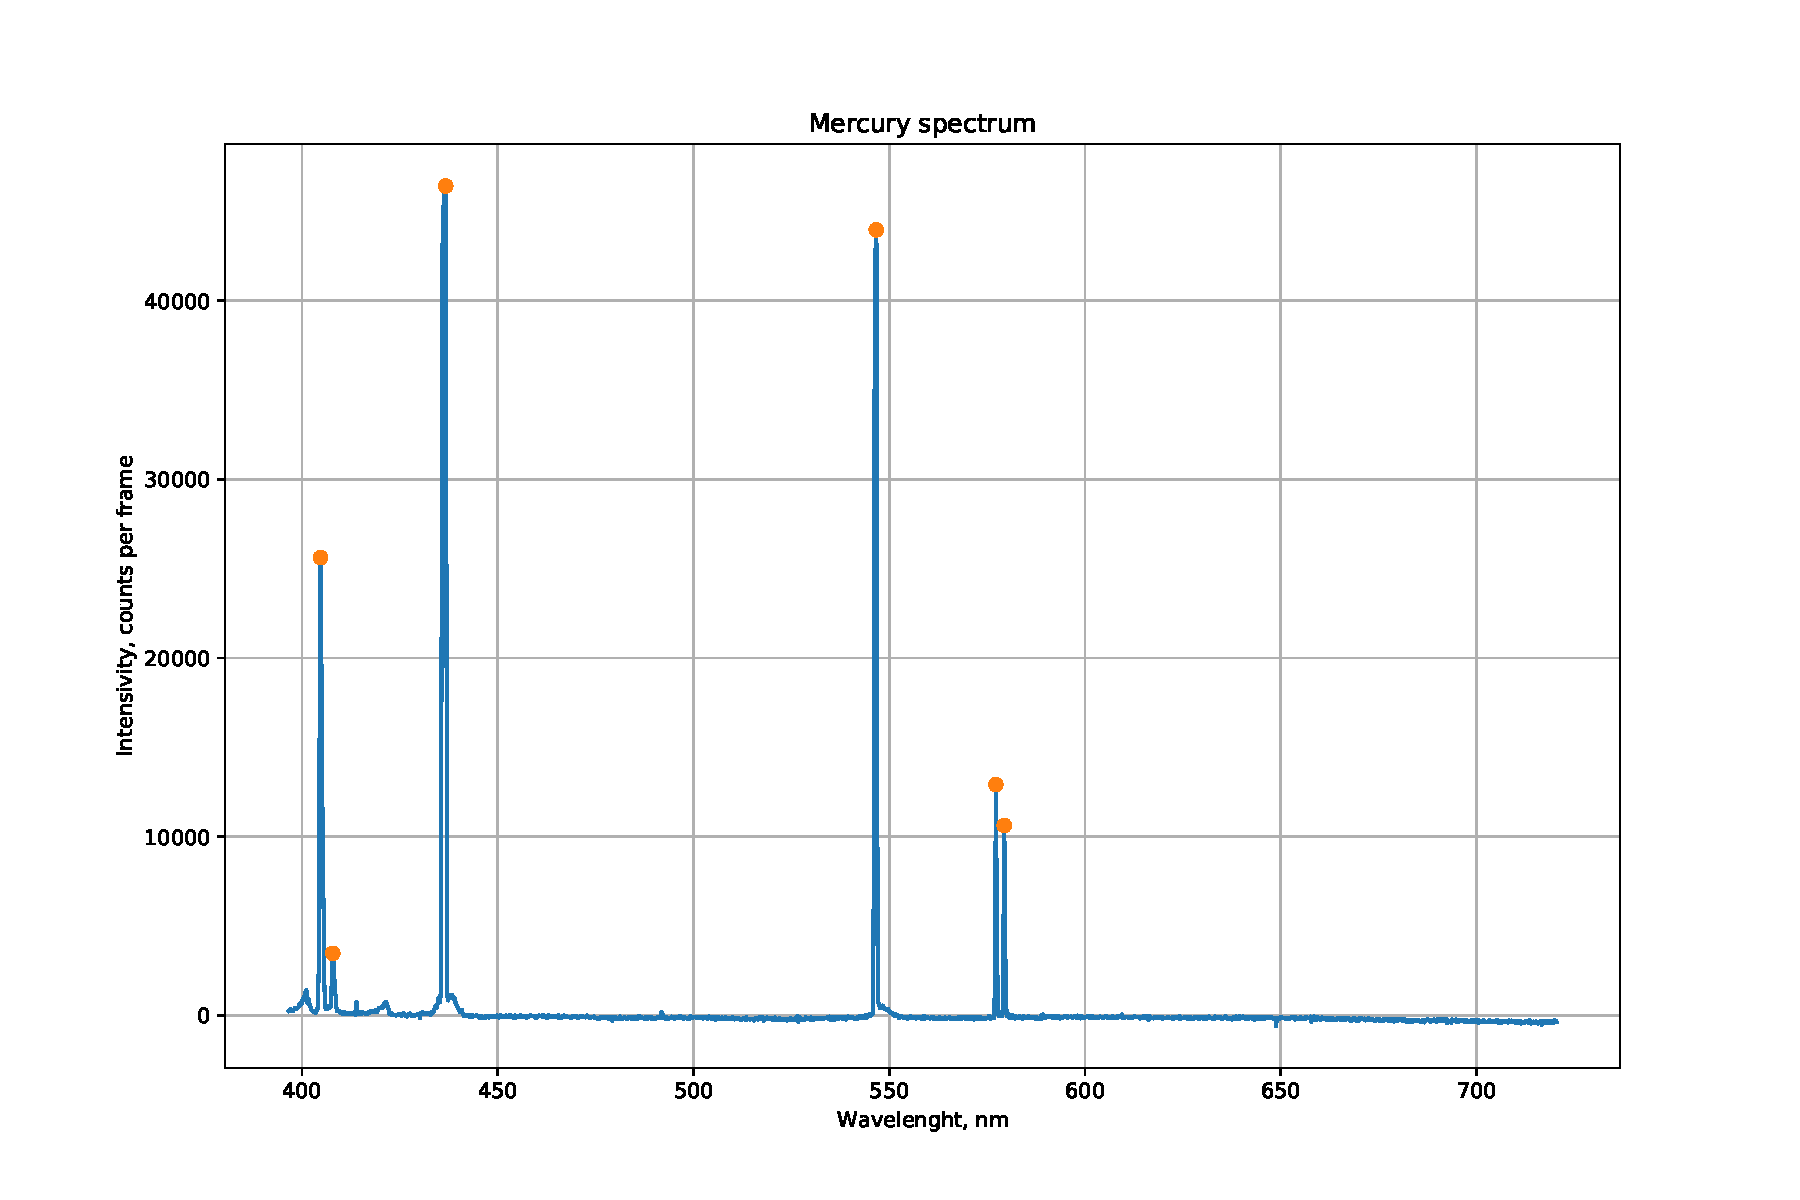
\includegraphics[width=0.9\linewidth]{mercury}
	\caption{Спектр ртути}
	\label{fig:hg}
\end{figure}

\begin{figure}[H]
	\centering
	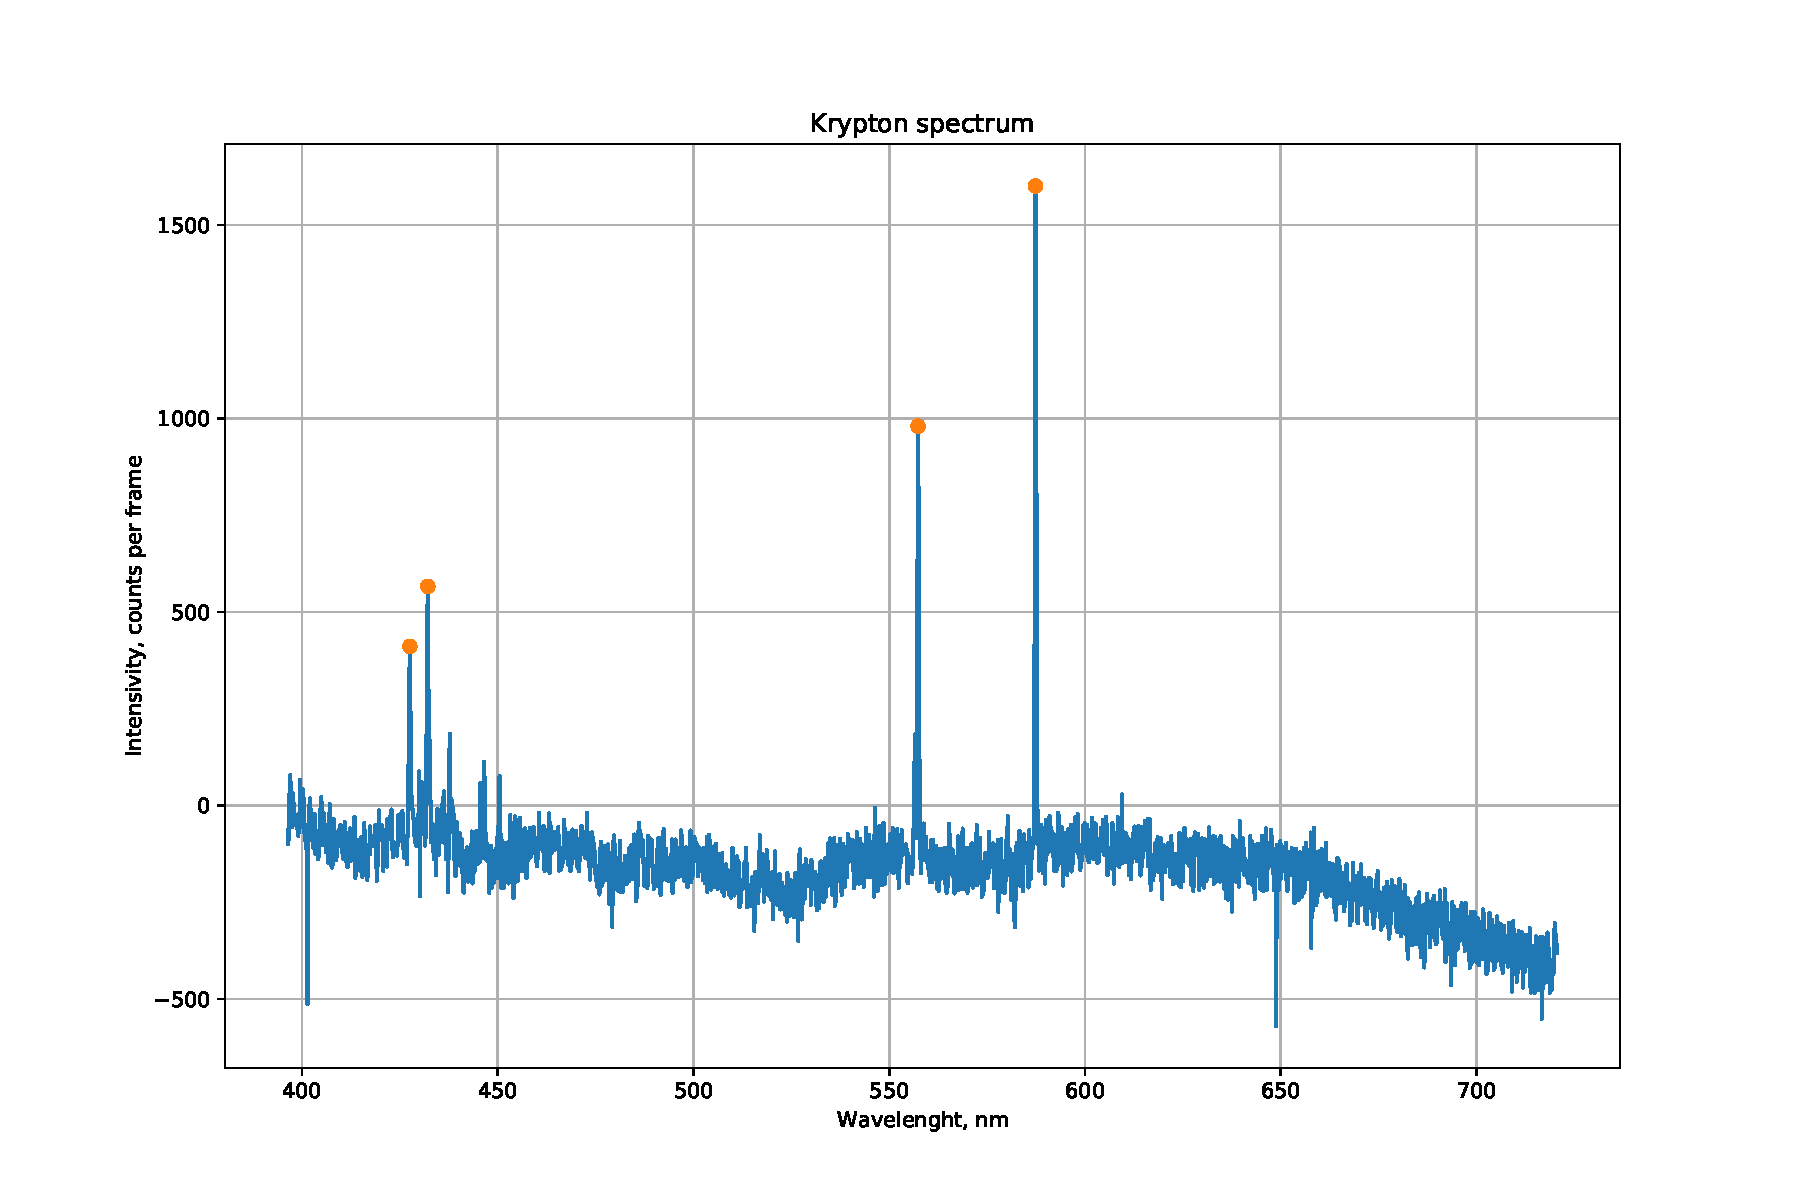
\includegraphics[width=0.9\linewidth]{krypton}
	\caption{Спектр криптона}
	\label{fig:kr}
\end{figure}

\begin{figure}[H]
	\centering
	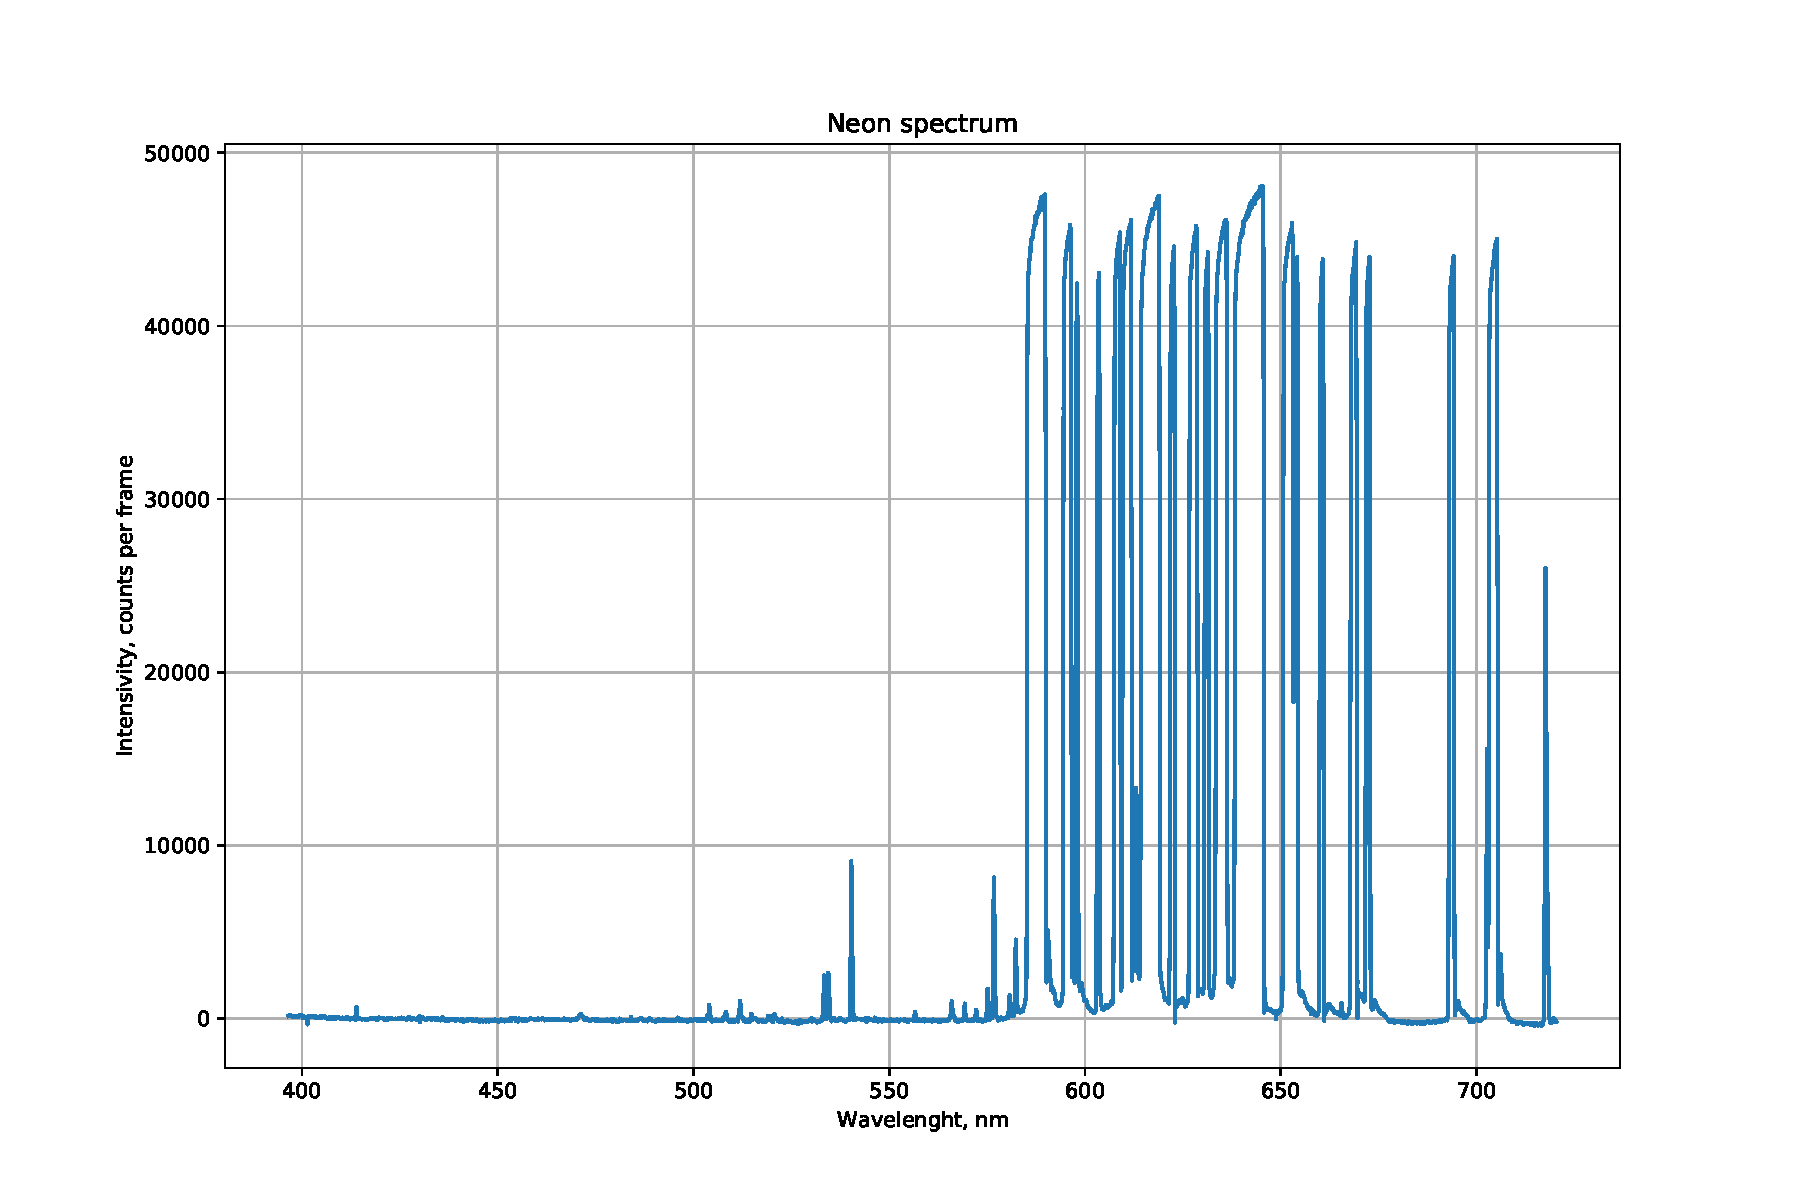
\includegraphics[width=0.9\linewidth]{neon}
	\caption{Спектр неона}
	\label{fig:ne}
\end{figure}

\begin{figure}[H]
	\centering
	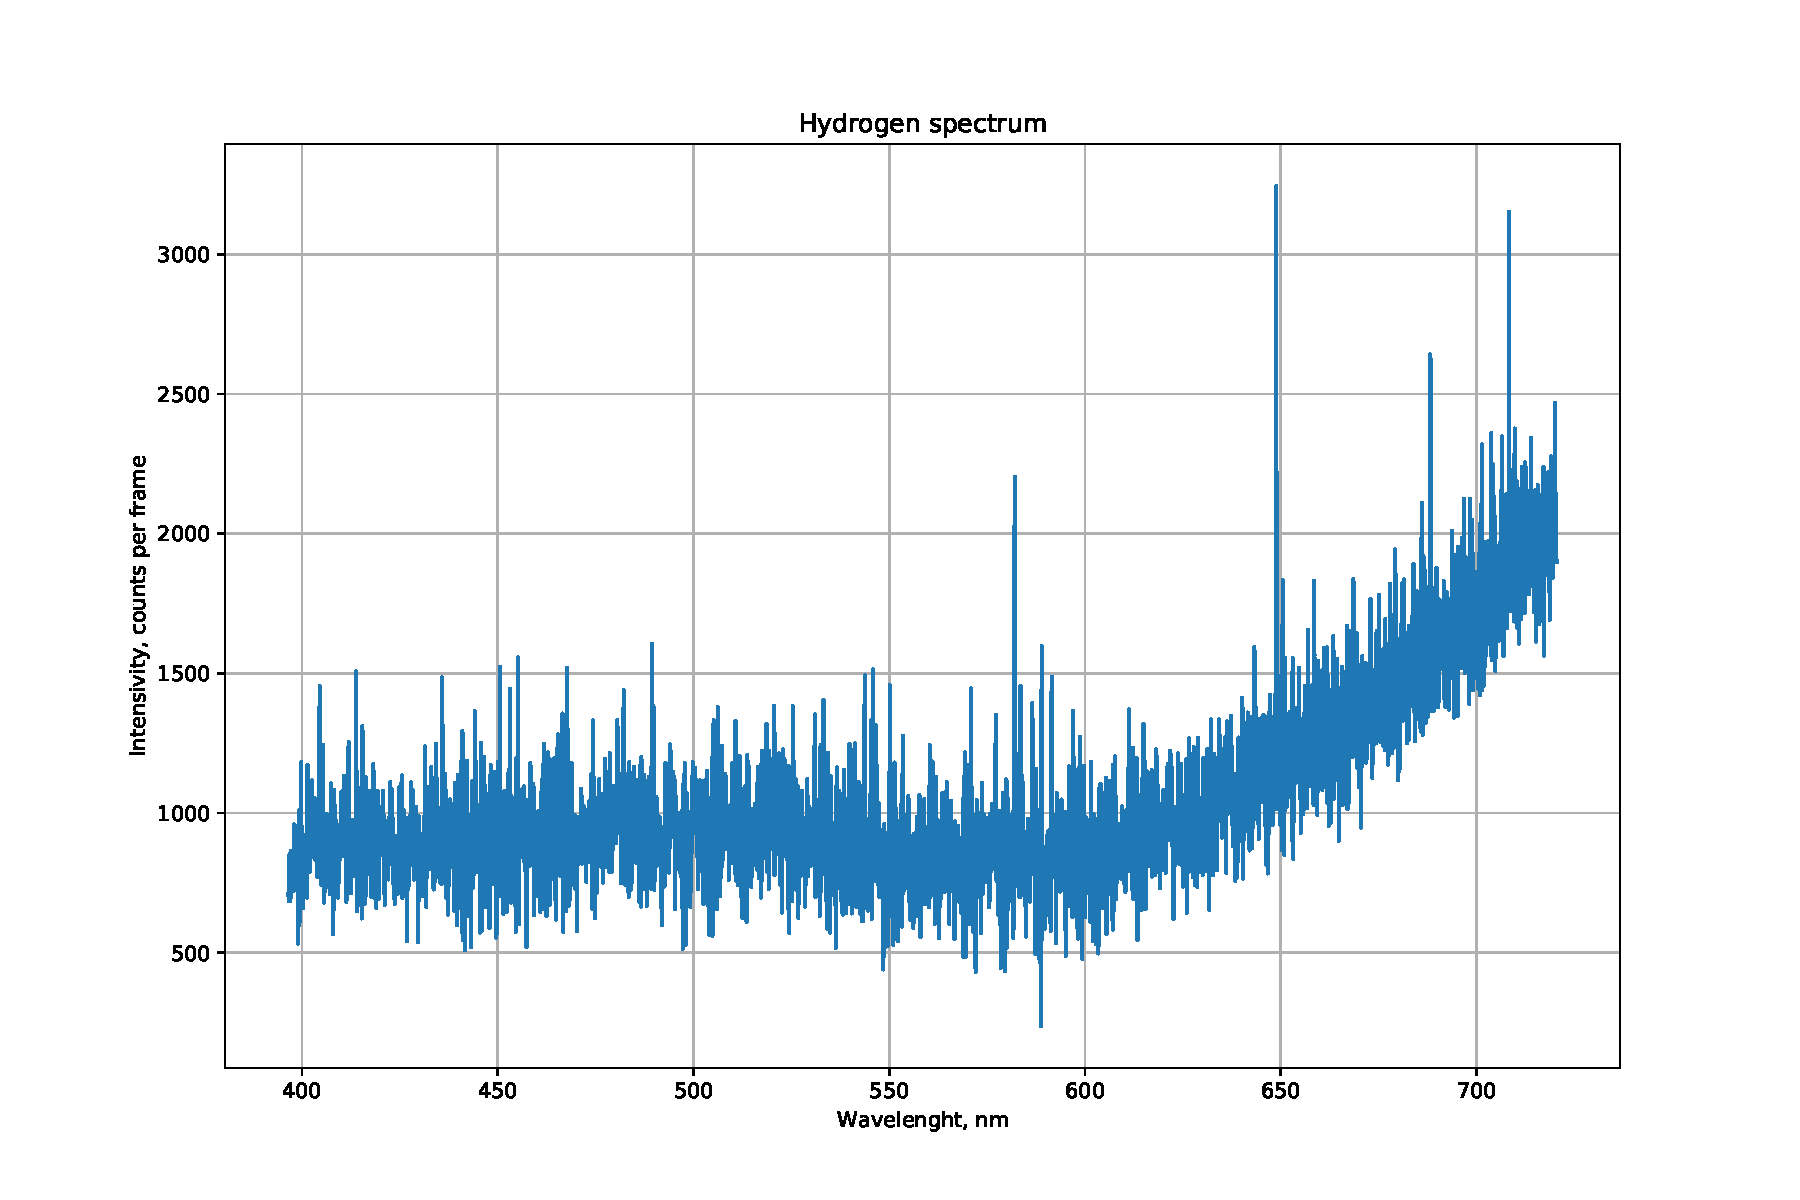
\includegraphics[width=0.9\linewidth]{h2}
	\caption{Спектр водорода}
	\label{fig:h2}
\end{figure}

\begin{figure}[H]
	\centering
	
\includegraphics[width=0.9\linewidth]{na}
	\caption{Спектр натрия}
	\label{fig:na}
\end{figure}

% 2

\begin{figure}[H]
	\centering
	
\includegraphics[width=0.9\linewidth]{sky_spectrum}
	\caption{Спектр серого неба напрямую (рыжий) и через оконное стекло (голубой)}
	\label{fig:sky}
\end{figure}

\begin{figure}[H]
	\centering
	
\includegraphics[width=0.9\linewidth]{glass_permeability}
	\caption{Зависимость коэффициента пропускания оконного стекла от длины волны}
	\label{fig:glass_perm}
\end{figure}

% 3

\begin{figure}[H]
	\centering
	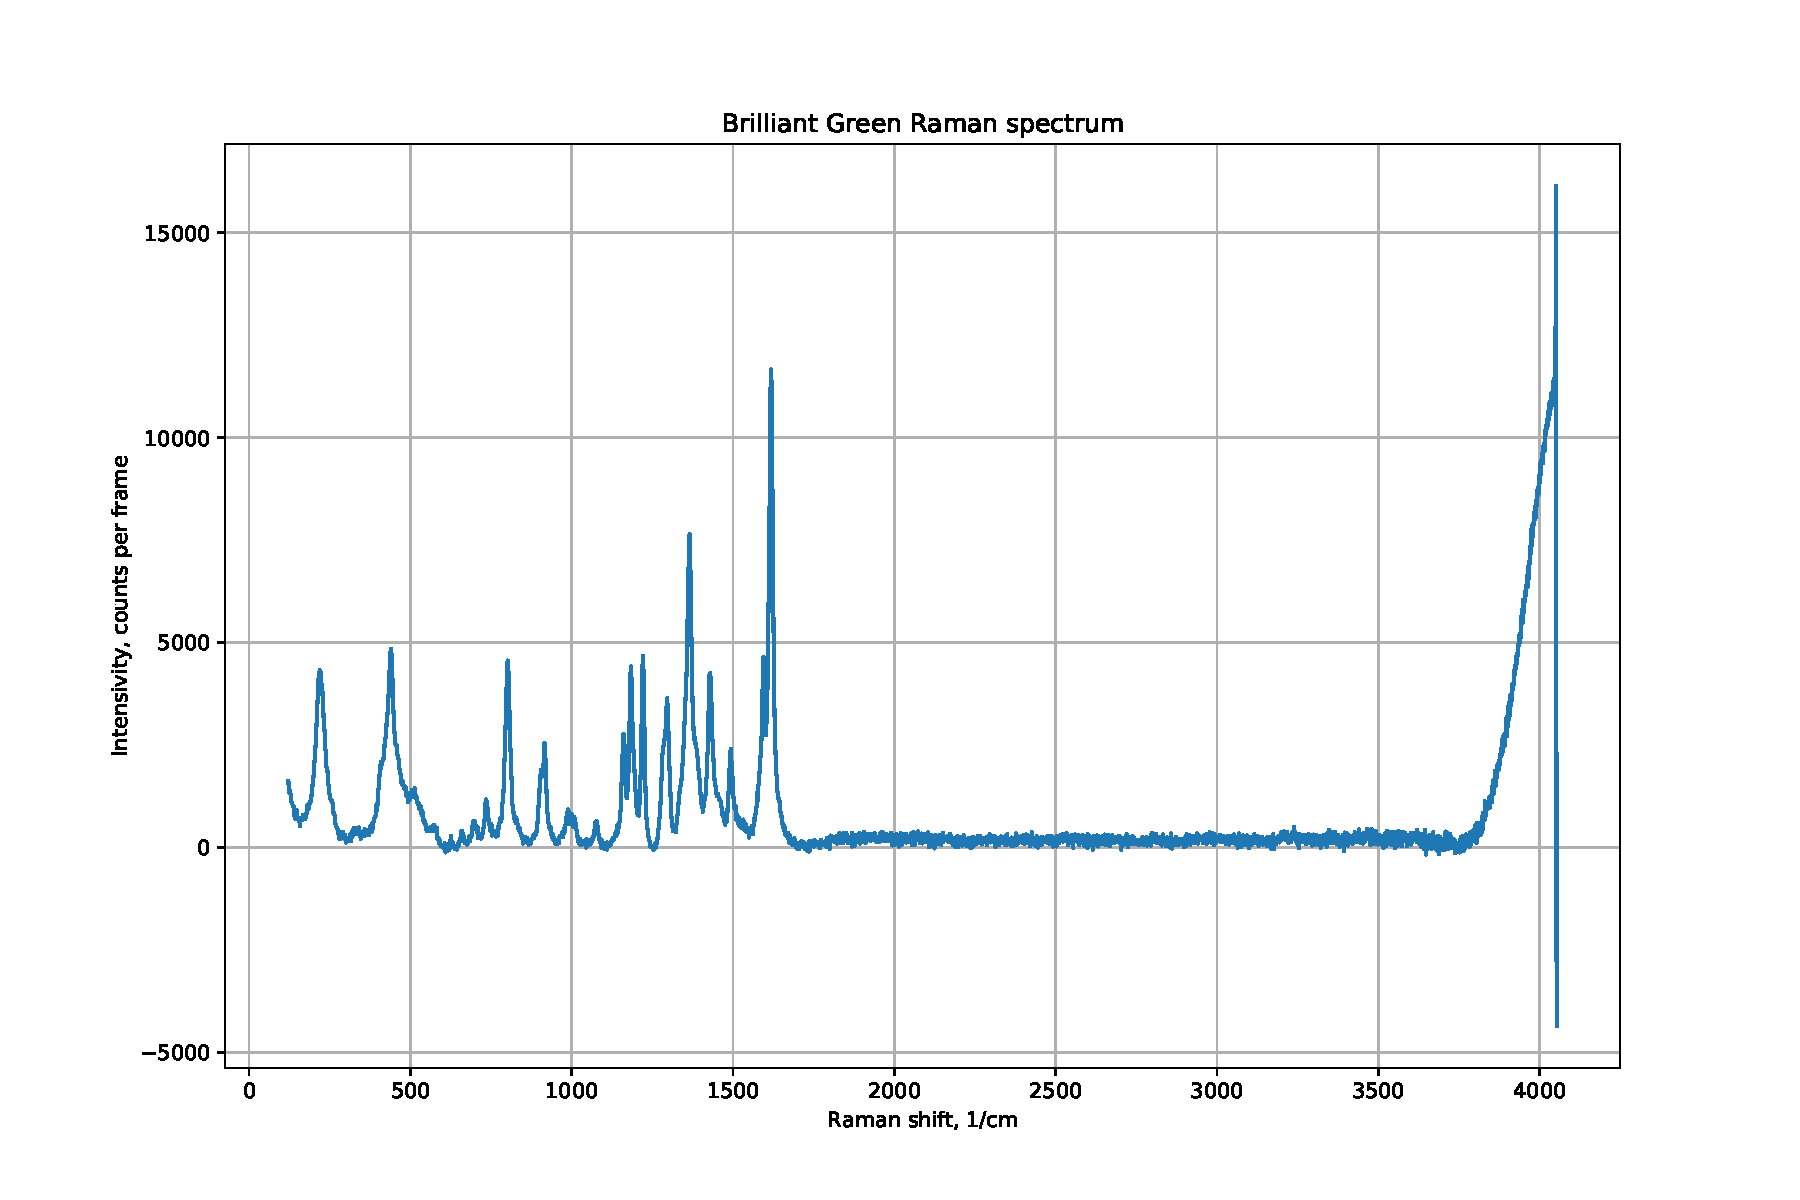
\includegraphics[width=0.9\linewidth]{raman_brilliant_green}
	\caption{Рамановский спектр зеленки}
	\label{fig:br_gr}
\end{figure}

\begin{figure}[H]
	\centering
	
\includegraphics[width=0.9\linewidth]{raman_water}
	\caption{Рамановский спектр воды}
	\label{fig:water}
\end{figure}

\begin{figure}[H]
	\centering
	
\includegraphics[width=0.9\linewidth]{raman_chalk}
	\caption{Рамановский спектр мела}
	\label{fig:chalk}
\end{figure}

\begin{figure}[H]
	\centering
	
\includegraphics[width=0.9\linewidth]{raman_coffee}
	\caption{Рамановский спектр кофеина в таблетках}
	\label{fig:coffee}
\end{figure}

\begin{figure}[H]
	\centering
	
\includegraphics[width=0.9\linewidth]{raman_validol}
	\caption{Рамановский спектр валидола}
	\label{fig:validol}
\end{figure}







\end{document}